%
%  MP_talk.tex
%
%  Created by Steven Harms (HOME) on 2011-07-26.
%  Copyright (c) 2011 Steven G. Harms. All rights reserved.
%
\documentclass[slidestop,compress,mathserif,notes]{beamer}
% Toggle between 'notes' and no notes to display or undisplay notes pages

% \usepackage[bars]{beamerthemetree}
\usetheme{PaloAlto}
\usecolortheme{seahorse}

% Use utf-8 encoding for foreign characters
\usepackage[utf8]{inputenc}

% Surround parts of graphics with box
\usepackage{boxedminipage}

% Package for including code in the document
\usepackage{listings}

% This is now the recommended way for checking for PDFLaTeX:
\usepackage{ifpdf}

\ifx\pdftexversion\undefined
\usepackage[dvips]{graphicx}
\else
\usepackage{graphicx}
\DeclareGraphicsRule{*}{mps}{*}{}
\fi
\title{Practical Metaprogramming:  Modeling Thought}
\author{ Steven G. Harms }

\date{2011-08-12}

\begin{document}

\ifpdf
\DeclareGraphicsExtensions{.pdf, .jpg, .tif}
\else
\DeclareGraphicsExtensions{.eps, .jpg}
\fi


\section{Introduction} % (fold)
\label{sec:introduction}
\begin{frame}
	\maketitle
\end{frame}

\subsection{Administration}
\begin{frame}
	\frametitle{Contact Me!}
	\begin{center}
		Steven G. Harms \\
		\vskip 1.25cm	
		Physically:  San Francisco, CA\\
		Email:  \texttt{lsrcv@sgharms.oib.com} \\
		Twitter / GitHub:  \texttt{sgharms} \\
		G+
	\end{center}
\end{frame}

\note{
Good afternoon, I want to welcome you all to the first day of Lone Star Ruby
Conference V. 
}

\begin{frame}
	\frametitle{Austin}
	\begin{center}
		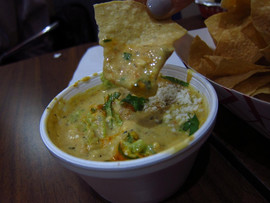
\includegraphics[scale=0.75]{img/queso.JPG}	
	\end{center}
	
\end{frame}
\note{
It's great to be back here in Austin. I've lived here for over
eight years off and on and love this town, its vibrant Ruby community, and
creativity with turning cheese into a soup that you put chips in. If you don't
know what I'm talking about, talk to me later and we'll get you set up
properly.
}
% section introduction (end)

\begin{frame}
	\frametitle{SpeakerRate}
	\centering{Help me Get Better!}
	\vskip 1.25cm
	\centering{\texttt{http://speakerrate.com/talks/\\7831-practical-metaprogramming-modeling-thought}}
\end{frame}

\subsection{Overview}

\begin{frame}
	\frametitle{What We'll Cover}
	Practical Programming:  Modeling Thought
\end{frame}

\begin{frame}
	\frametitle{What we'll cover cont'd}
	\textbf{OR}:Lessons Learned While Using Ruby's MP System to Model a 2,500 Year-Old, Dead Language 
\end{frame}
\note{
In all seriousness, I want to give you all a bit of an overview of what we're
going to talk about today. Let's first talk about Practical Metaprogramming.
}


% Use this at Rubyconf
% \begin{frame}
% 	\frametitle{``Long Title''}
% 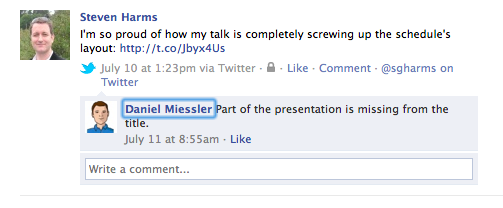
\includegraphics[scale=0.55]{img/daniel_comment.png}	
% \end{frame}
% \note{
% In all seriousness, I want to give you all a bit of an overview of what we're
% going to talk about today. Let's first talk about Practical Metaprogramming.
% }

\begin{frame} 
	\frametitle{``Practical Metaprogramming:  First Contact''}
  ``How do we start exploring MP in Ruby?''

	
\includegraphics[scale=0.55]{img/first_contact.jpg}
\end{frame} 
\note{

}

\begin{frame} \frametitle{``Practical Metaprogramming''}

 	\begin{itemize} 
		\item \texttt{attr\_*}Z \emph{Page 30}
  \end{itemize}
	\vskip 0.5cm
	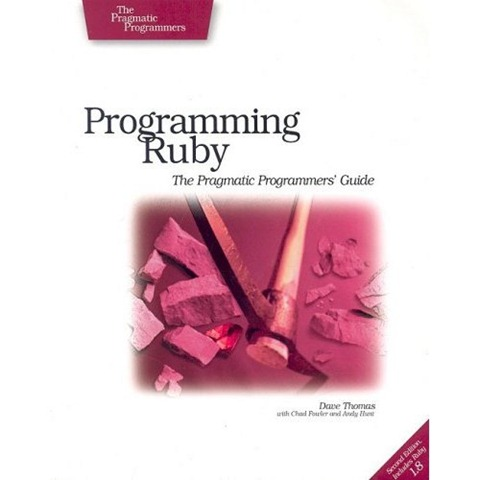
\includegraphics[scale=0.45]{img/ruby_pickaxe.jpg}	
\end{frame} 
\note{For many Ruby developers, our first exposure to the world of
Metaprogramming starts around page thrity of the PickAxe book when we are
introduced to attr\_reader, attr\_writer, and attr\_accessor. For those of us
coming rom Java ,the ability to be able to have attributes' accessors and
mutators be provided for us is one of the things that makes us go ``Ooh!''
about Ruby.  In my edition of the Pickaxe book, this first appeared on page
30.
}

\begin{frame} \frametitle{``Practical Metaprogramming''}

 \begin{itemize} 
	\item \texttt{attr\_*}:  \emph{Page 30}
	\item Rails (\texttt{order.discount=0.5}):  \emph{Page 28}
\end{itemize}
	\begin{center}
		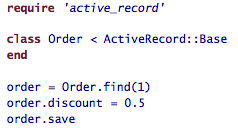
\includegraphics[scale=0.55]{img/awdwr_mp.png}	
	\end{center}
	
\end{frame}

\note{ Further, given that many people come to Ruby \emph{via} Rails, Rails
asks us to accept a great many things as ``magic'' as we get underway with it.
Rails first presents MP on page 28 in the context of how ActiveRecord maps
database fields to instance variables in its object-relational mapping.
}


\begin{frame}
	\frametitle{``Practical Metaprogramming''}
	\begin{itemize} 
		\item \texttt{attr\_*}:  \emph{Page 30}
		\item Rails (\texttt{ORM}):  \emph{Page 28}
	\end{itemize}
\end{frame}

\note{This is generally a suitable beginning and once we accept that we live in
a world laced with metaprogramming magic, we're generally content to simply
inhabit it. If we start to explore more about Metaprogramming, we start to
move to a place that, I contend, is generally \emph{impractical}.}

\begin{frame}
	\frametitle{``Slightly Impractical Metaprogramming:''  Open Classes}
	\begin{itemize}
		\item Open Classes
	\end{itemize}
		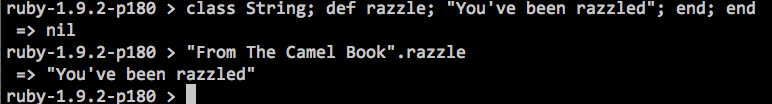
\includegraphics[scale=0.45,width=10cm,height=2cm]{img/open_class.png}	
\end{frame}
\note{It usually starts like this. You realize that you can add methods to an
existing class and add ``interesting'' features to classes. \emph{Describe
``Open Class''}. Incidentally I have taken these names from the nomenclature
provided by Paolo Perrotta's book with Pragmatic Press: Metaprogramming Ruby.
I'll provide a link to that book as well as to a gist, published by Paolo,
that has copy-able code available at GitHub}

\begin{frame}
	\frametitle{``Slightly Impractical Metaprogramming:''  Kernel Method}
	\begin{itemize}
		\item Open Classes
		\item Kernel Method
	\end{itemize}
		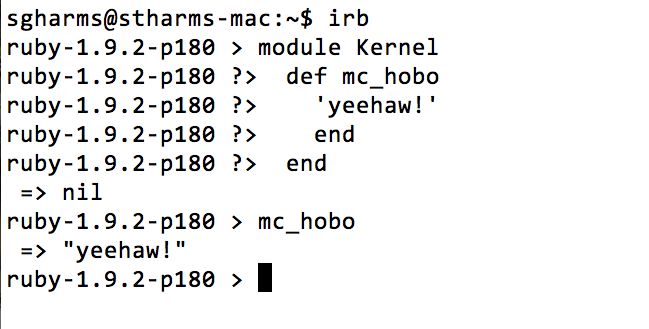
\includegraphics[scale=0.55]{img/kernel_method.png}	
\end{frame}
\note{At this point we're starting to feel some power here and we'll start to
do some interesting work. Although from my entirely unscientific survey,
here's the one that we Rubyists love to show Java programmers}

\begin{frame}
	\frametitle{``Slightly Impractical Metaprogramming:  Singleton Method''}
	\begin{itemize}
		\item Open Classes
		\item Kernel Method
		\item Singleton Method
	\end{itemize}
		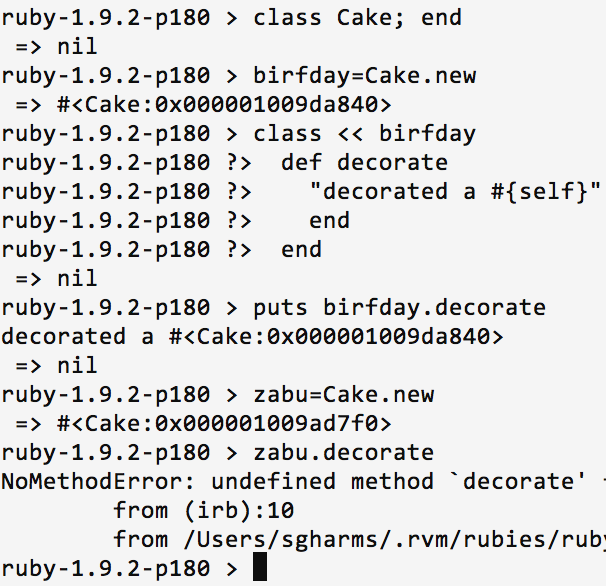
\includegraphics[scale=0.35]{img/singleton_method.png}
\end{frame}
\note{This is undoubtedly the one that makes the pro-Java camp weep. In
compiled languages the definition of a class represents a contract of sorts,
between you and the compiler. A class is an expression of that contract. In
Ruby, a class is really a namespace expression.  This is pretty cool stuff.}

\begin{frame}
		\frametitle{AWESOMENESS}
		\begin{center}
			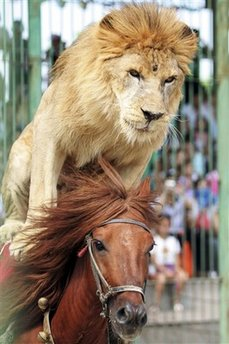
\includegraphics[scale=0.45]{img/lion_horse.jpg}
		\end{center}			
\end{frame}
\note{It might not be the most awsome thing ever, which is, of course, a lion riding a horse, but it's still pretty good.}

\begin{frame}
	\frametitle{Madness}
	This leads to the dangers of MP:
	\begin{itemize}
		\item Opaqueness
		\item Unpredictability
		\item Unsupportability
	\end{itemize}
	\begin{center}
			\emph{Abandon all hope ye who enter \ldots}
		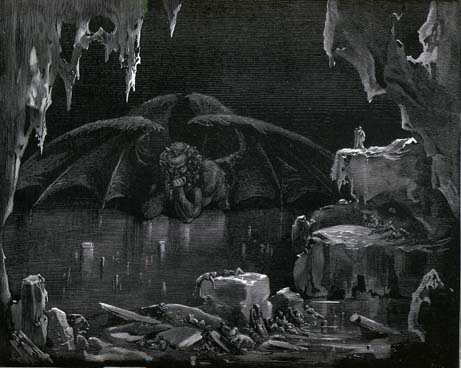
\includegraphics[scale=0.45]{img/dante.jpg}		
	\end{center}
\end{frame}

\begin{frame}
	\frametitle{F.U.D.}
		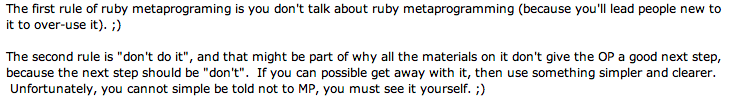
\includegraphics[width=0.98\textwidth, height=0.25\textheight]{img/tim_hates_mp.png}		
		\vskip 0.5cm
		\emph{--Tim Connor:  SF Ruby Mailing List}
\end{frame}

\begin{frame}
	\frametitle{anti-F.U.D.}
		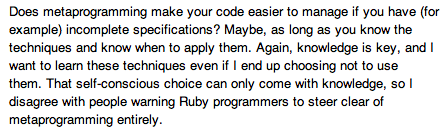
\includegraphics[width=0.98\textwidth, height=0.45\textheight]{img/paolo_anti_fud.png}		
		\vskip 0.5cm
		\emph{--Paolo Perrotta, author of Metaprogramming Ruby, in e-mail to Steven Harms}
\end{frame}

\begin{frame}
	\frametitle{What this talk will do:}
	\begin{itemize}
		\item Practical Metaprogramming: Move you beyond the F.U.D. around Metaprogramming
	\end{itemize}
\end{frame}

\begin{frame}
	\frametitle{What this talk will do:}
	\begin{itemize}
		\item Practical Metaprogramming: Move you beyond the F.U.D. around Metaprogramming
		\item Modeling Thought:  A guideline for identifying ideal cases for Metaprogramming
	\end{itemize}
\end{frame}

\begin{frame}
	\frametitle{What this talk will do:}
	\begin{itemize}
		\item Practical Metaprogramming: Move you beyond the F.U.D. around Metaprogramming
		\item Modeling Thought:  A guideline for identifying ideal cases for Metaprogramming
		\item Use examples from my LatinVerb library
	\end{itemize}
\end{frame}

% \begin{frame}
% 	\frametitle{VALETE!}
% 	\begin{center}
% 		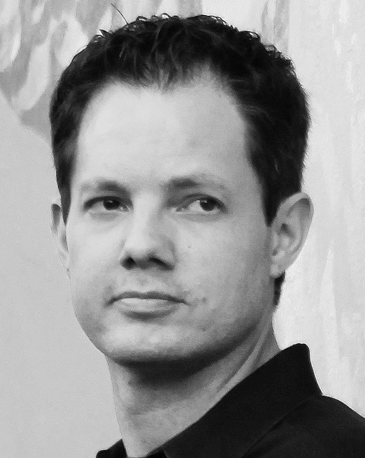
\includegraphics[scale=0.25]{img/wynn.png}			
% 	\end{center}
% 	\emph{Maybe you want to learn about mobile development with Wynn\ldots}
% 	
% \end{frame}
\note{
That's the lay of the land for this talk. If you're thinking this talk might
not be for you, then you're welcome to hop over. 
}

\begin{frame}
	\frametitle{Socially Awkward Penguin}
	\begin{center}
		
\includegraphics[scale=0.3]{img/sap.png}			
	\end{center}	
\end{frame}
\note{
Whew, I'm glad we only lost those few. 
}

\begin{frame}
	\frametitle{Forever Alone}
	\begin{center}
		
\includegraphics[scale=0.25]{img/forever_alone.png}
	\end{center}
\end{frame}

\begin{frame}
	\frametitle{``Impractical'' to ``Practical'' Metaprogramming}	
  34 ``Spells''
\end{frame}
\note{
Earlier I suggested that the problem was that when we learned the various
MP techniuqes, we were learning tools or gimmicks. Accordingly, you can't
build something great, an edifice of importance out of a gimmick. }

\begin{frame}
	\frametitle{``Impractical'' to ``Practical'' Metaprogramming}	
		34 ``Spells''
		\begin{center}
			\tiny
			\begin{tabular}{|c|c|c|c|}
				\hline
				Argument Array & 
				Around Alias & 
				Blank Slate & 
				Class Extension \\
		
				\hline			
				Class Extension Mixin &
				Clean Room & 
				Code Processor &
				Context Probe \\
				
				\hline
				Deferred Evaluation & 
				Dynamic Dispatch &
				Flat Scope & 
				Ghost Method \\ 
				
				\hline			
				Hook Method & 
				Kernel Method &
				Lazy Instance Variable &
				Named Arguments \\

				\hline
				Namespace & 
				Nil Guard & 
				Object Extension & 
				Pattern Dispatch  \\

				\hline
				Sandbox &
				Scope Gate & 
				Self Yield & 
				Shared Scope \\

				\hline
				Singleton Method &
				String of Code & 
				Open Class & 
				Symbol to Proc \\

				\hline			
				Class Instance Variable  & 
				Class Macro &
				Dynamic Method & 
				Dynamic Proxy  \\

				\hline
				Mimic Method &
				Monkeypatch \\
				\hline
			\end{tabular}
		\end{center}
		\normalsize
		\vskip 0.5cm
		\emph{Source:  \underline{Metaprogramming Ruby}}
\end{frame}
\note{
Thanks to Paolo's work, there are now 34 possible formulae available. If by
having one hammer, everything starts to look like a nail, it's unsurprising
that when you have 34 hammers, you indulge in finding 34 ways to use hammers.

And this is probably the reason for our friend Tim to take a fairly hard line
against MP, as we saw earlier.

A house is not several thousand home improvement projects. A house is a vision
whose execution requires that amount of work.

In consideration of these thrity-four opportuntites for misdirection, let's
try to come up with a unified vision of what makes certain situations call for
a metaprogrammatic solution. }

\begin{frame}
	\frametitle{Harms' First Law of Metaprogramming}
	\centering{\emph{	A metaprogrammatic solution is suitable when you need to provide
	unambiguous answers (return values) to ambiguously asked things (flexible /
	incomplete method calls)}
}\end{frame}

\begin{frame}
	\frametitle{Harms' First Law of Metaprogramming}
	\centering{\emph{	A metaprogrammatic solution is suitable when you need to provide
	unambiguous answers (return values) to ambiguously asked things (flexible /
	incomplete method calls)}
	\vskip 0.5cm
	\centering{\emph{e.g. Rails' ORM Calculation}}
}\end{frame}

\begin{frame}
	\frametitle{Harms' Second Law of Metaprogramming}
	\centering{\emph{	A metaprogrammatic solution is suitable when typing the syntax required would totally suck}}
	\vskip 0.5cm
	\centering{\emph{e.g. attr\_* methods}}
\end{frame}

\begin{frame}
	\frametitle{Harms' First Corrolary:}
	\begin{center}
		\emph{Any significant metaprogramming work undertaken to meet either of the laws will eventually look like it was undertaken for a reason in service to the opposite law}
	\end{center}
\end{frame}

\section{Modeling Thought} % (fold)
\label{sec:modeling_thought}


\begin{frame}
	\frametitle{``Modeling Thought''}
	\large
	\centering{First Law \\ + \\ Second Law \\ = \\ }
	\vskip 0.5cm
	\begin{center}
		``Modeling Thought''
	\end{center}
	
	\normalsize
\end{frame}
\note{

``Modeling Thought'' is a name for evaluating when MP is a good idea. If we
aggregate the first law and the second law, we start to see that they are
exactly descripitve of two important qualities of the way humans think.

That is, human minds are very good at the formation of heuristics based on
patterns that Rubyists would recognize like \texttt{Enumerable\#map} or
\texttt{Enumerable\#grep} so that instead of having to memorize thousands of
discrete rules, we can operate a heuristic to generate the answers.

Similarly, humans are very good at receiving a partial representation of a
reference to a data-set and understanding whether a unique data-set is being
requested, or if we can represent the data sought in a smaller format or in a
shorter format.
}

\begin{frame}
	\frametitle{``Modeling Thought: Born That Way''}
	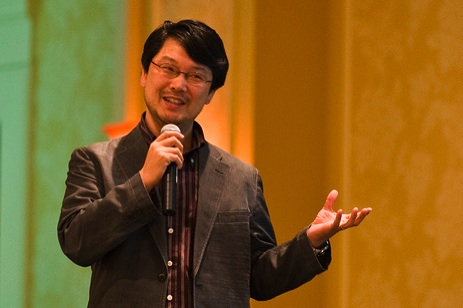
\includegraphics[scale=0.6]{img/matz.jpg}		
\end{frame}
\note{
And no language supports the ``modeling thought'' paradigm like Ruby. By
providing a language that gives rise to the 30-odd ``Spells'' limned by
Perrotta, and under guidance of ``Modeling Thought\'s'' paradigms we can
safely decide whether we are using or abusing Ruby's metaprogramming
capabilities. We can mitigate the grounds for Tim's FUD around MP's
sensibility.

In this case you're modeling with human's thought processes before the syntax
rules of the language. 
}

\begin{frame}
	\frametitle{Reification of ``Modeled Thought'' is Language}
	\begin{itemize}
		\item No problem domain exemplifies this problem as well as human language.
	\end{itemize}	
\end{frame}

\begin{frame}
	\frametitle{\textsc{LATIN}}
	\begin{itemize}
		\item Dead:  \emph{Easier to hit a still target}
	\end{itemize}
\end{frame}

\begin{frame}
	\frametitle{\textsc{LATIN}}
	\begin{itemize}
		\item Dead:  \emph{Easier to hit a still target}
		\item Highly-Regular:  (\textasciitilde3-5 truly irregular verbs)
	\end{itemize}
\end{frame}

\begin{frame}
	\frametitle{\textsc{LATIN}}
	\begin{itemize}
		\item Dead:  \emph{Easier to hit a still target}
		\item Highly-Regular:  (\textasciitilde3-5 truly irregular verbs)
		\item Well-documented:  (Since \textasciitilde75 BCE)
	\end{itemize}
\end{frame}

\begin{frame}
	\frametitle{\textsc{LATIN}}
	\begin{itemize}
		\item Dead:  \emph{Easier to hit a still target}
		\item Highly-Regular:  (\textasciitilde3--5 truly irregular verbs)
		\item Well-documented:  (Since \textasciitilde75 BCE)
		\item Defined by heuristic:  \emph{Wheelock}
	\end{itemize}
\end{frame}

\begin{frame}
	\frametitle{Just Enough Latin}
	\vskip 0.5cm
	``Captain!  My Captain!''
\end{frame}

\begin{frame}
	\frametitle{How can we see ``Modeled Thought'' in \textsc{LATIN}?} 
	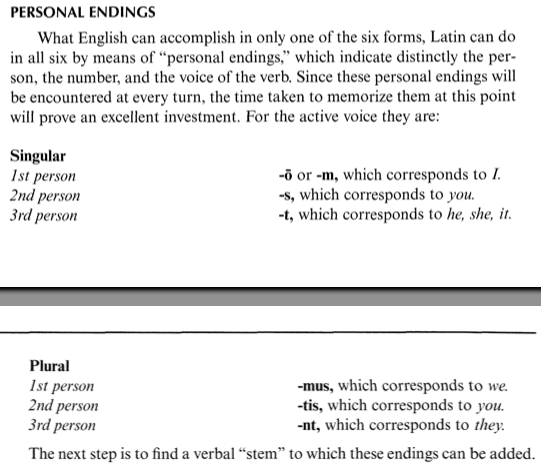
\includegraphics[scale=0.45]{img/conj_how_1.png}
\end{frame}

\begin{frame}
	\frametitle{How can we see ``Modeled Thought'' in \textsc{RVBY}?} 
	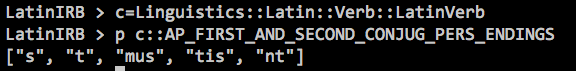
\includegraphics[scale=0.45]{img/conj_how_1b.png}
\end{frame}


\begin{frame}
	\frametitle{How can we see ``Modeled Thought'' in \textsc{LATIN}?} 
	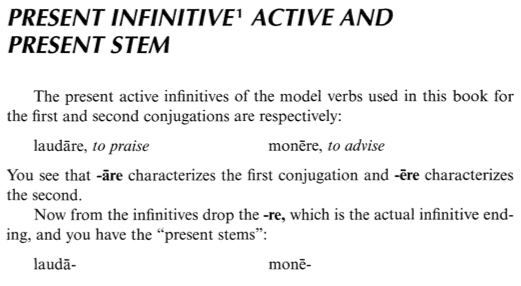
\includegraphics[scale=0.45]{img/conj_how_2.png}
\end{frame}

\begin{frame}
	\frametitle{How can we see ``Modeled Thought'' in \textsc{RVBY}?} 
		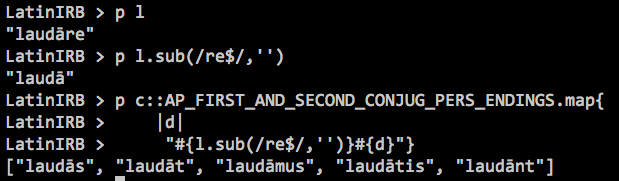
\includegraphics[scale=0.45]{img/conj_how_2b.png}	
\end{frame}


\begin{frame}
	\frametitle{How can we see ``Modeled Thought'' in \textsc{LATIN}?} 
	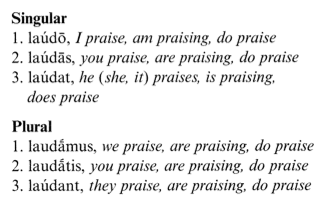
\includegraphics[scale=0.45]{img/conj_how_3.png}	
\end{frame}

\begin{frame}
	\frametitle{How can we see ``Modeled Thought'' in \textsc{RVBY}?} 
	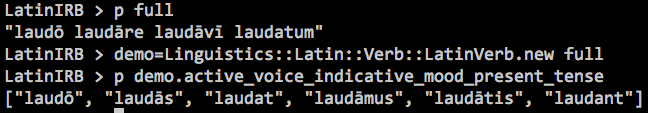
\includegraphics[scale=0.45]{img/conj_how_3b.png}	
\end{frame}

\begin{frame}
	\frametitle{Placeholder}
	\ldots
\end{frame}

\subsection{Repetition} % (fold)
\label{sub:repetition}

\begin{frame}
	\frametitle{Placeholder}
	\ldots
\end{frame}


% subsection repetition (end)

\subsection{Methods} % (fold)
\label{sub:methods}

\begin{frame}
	\frametitle{Placeholder}
	\ldots
\end{frame}

\subsubsection{De-parameterize}

\begin{frame}
	\frametitle{Placeholder}
	\ldots
\end{frame}


\subsubsection{Embed Parameters in Method Calls}

\begin{frame}
	\frametitle{Placeholder}
	\ldots
\end{frame}

% subsection methods (end)

\subsection{Domain-Specific Languages} % (fold)
\label{sub:domain_specific_languages}
\begin{frame}
	\frametitle{Placeholder}
	\ldots
\end{frame}

% subsection domain_specific_languages (end)

% section modeling_thought (end)

\section{Supplementary} % (fold)
\label{sec:supplementary}

\begin{frame}
	\frametitle{Book}
	\underline{Metaprogramming Ruby} by Paolo Perrotta
\end{frame}

\begin{frame}
	\frametitle{Gist}
	
	
\end{frame}

% section supplementary (end)

\end{document}

